% !TEX root =  ../main.tex
\section{Among}
\subsection{Definition}

\subsubsection{Signature} \cstr{among(vs : set<VM>, ns : set<set<server>>)}

\begin{itemize}
\item \cstr{vs} : an non-empty set of VMs for a meaningful constraint. VMs not in the \st{Running} state are ignored.
\item \cstr{ns} :  an non-empty set of set of servers or the constraint is sure of not being satisfiable.
Sets composing \cstr{ns} must be disjoint. Servers not in the \st{Online} state are ignored.
\end{itemize}

The \cstr{among} constraint forces each running VM in \cstr{vs} to be hosted on one of the set of servers in \cstr{ns}.

\classification{among}{application administrator,datacenter administrator}{VM placement}{Partitioning,VM-to-VM placement,VM-to-server placement,Performance}


\subsubsection{Usage}

The \cstr{among} constraint may be used by a datacenter administrator or
an application administrator to group closely related VMs with regards to specific criteria.
%
A datacenter network is usually designed as a fat-tree~\cite{leiserson1985fat,al2008scalable} that
provides a non-uniform network latency and bandwidth between the servers.
An application administrator having strongly communicating VMs may then require
to have its VMs hosted on servers connected to a same edge switch to improve
their communication. This  can be achieved using one \cstr{among} constraint
where each set of servers denotes the servers connected to a same edge switch.

A datacenter administrator may also rely on \cstr{among} constraints to part the datacenter
and ease its management.
%
First, the administrator reflects, using disjoint set of servers, the current physical partitioning (different geographical sites, administrative zones, shipping containers of servers~\cite{containers}, \dots) of the datacenter.
%
\cstr{Among} constraints are then use to force groups of VMs to stay inside a single physical
partition.
 

\subsubsection{Example}

Figure~\ref{lst: among} depicts a sample reconfiguration between a source and a destination configuration.
In this example, the following \cstr{among} constraints were considered:

\begin{itemize}
\item \cstr{among(\{VM1, VM2, VM3\}, \{\{N1, N2\},\{N3, N4\}\})}. This constraint was not satisfied in the
source configuration as \cstr{VM1} and \cstr{VM2} were running on the partition \cstr{\{N1, N2\}}
while \cstr{VM3} was running on the partition \cstr{\{N3, N4\}}. The reconfiguration fixed this
violation by relocating \cstr{VM3} to \cstr{N2}. \cstr{VM2} was relocated to \cstr{N2} but this action
does not contradict the constraint.

\item \cstr{among(\{VM4, VM5\}, \{\{N1\},\{N2, N3, N4\}\})}. This constraint was not satisfied in the source configuration as \cstr{VM4} and \cstr{VM5} were running on distinct partitions. This violation was fixed by
suspending \cstr{VM5}.

\item \cstr{among(\{VM6, VM7\}, \{\{N1,N2\},\{N3, N4\}\})}. This constraint was already satisfied in the source configuration as both VMs were running on the partition \cstr{\{N1,N2\}}. The constraint is still satisfied in the destination configuration as both VMs have been relocated to the partition \cstr{\{N3,N4\}}.

\end{itemize}

\begin{reconfiguration}
\centering
\begin{minipage}[b]{0.40\textwidth}
\begin{lstlisting}
N1: VM1 VM2 VM6 VM7
N2: VM5
N3: VM3
N4: VM4 
\end{lstlisting}
\end{minipage}
\begin{minipage}[b]{2cm}
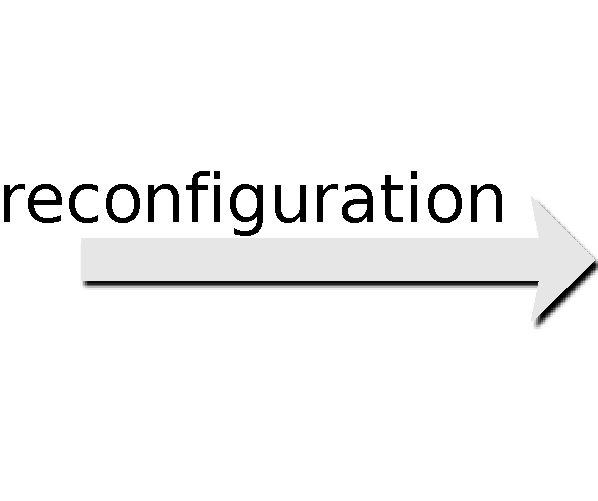
\includegraphics[width=2cm]{img/arrow_reconfiguration}
\end{minipage}
\begin{minipage}[b]{0.40\textwidth}
\begin{lstlisting}
N1: VM1 
N2: VM2 VM3 (VM5)
N3: VM6
N4: VM4 VM7
\end{lstlisting}
\end{minipage}
\caption{A reconfiguration motivated by \cstr{among} constraints.}\label{lst: among}
\end{reconfiguration}


\fullVersion{
\subsection{Model}

To implement \cstr{among}, each of the servers group is identified by a constant.
A variable $G$ is then created to indicate the group hosting the VMs. 
$G$ is linked to each of the d-slice placement variables to indicate
that if a d-slice of one of the given VM is hosted on a server, then all the VMs are
hosted on the set of servers to which this server belongs to. The equation~\eqref{eq: rp among}
depicts this model.
\todo{incorrect}
\begin{equation*}
\begin{split}
\text{\cstr{among}} & \text{\cstr{(V : set<VM>, S : set< set<server> >)}} \triangleq\\
& G \in <0.. card(S) - 1> \\
& \forall v_i \in V, d_i^{host} = j \imply 
G = j \leftrightarrow d_i^{host} \in S_j
\end{split}\label{eq: rp among}
\end{equation*}

\subsection{Availability}

\subsubsection{In {\btrp}}

The constraint \cstr{among}�is available in {\btrp}�since the version 2.1.
Each of the server groups is identified by a constant, and a variable is created to
indicate the selected group.  This variable is linked to each of the
d-slice placement variables using the \emph{nth} constraint, indicating
that if a d-slice of one of the given VM is hosted on a server, then all
the given VMs are hosted on the set of servers to which this server
belongs.

\subsection{Violation detection}

The \cstr{among} constraint restricts a VM placement relatively to the others.
If two VMs are assigned to different group of servers, it is then not possible
to detect which group is the \emph{right one}. To avoid to underestimate
the misplaced VMs, a safe approach consists in selecting every VMs
when they are placed on different group of servers. 
}


\subsection{See also}

\subsubsection{Related Constraints}
\begin{itemize}
\item \cstrref{fence}: The \cstr{fence} constraint is a specialization of the \cstr{among} constraint: only one set of servers is possible to restrict the VMs placement. A \cstr{among} constraint is then equivalent to a \cstr{fence} constraint when there is only one possible set of servers to host the VMs. This  occurs when only one set of servers is specified, when other sets are offline, or when one of the given VMs is ensured to be hosted on a known server as the other VMs will necessarily be hosted on the set of servers the known server belong to.

\end{itemize}
\emulatedWith{among}{splitAmong}{\cstr{among(vs1, ns1)}}{\cstr{splitAmong(\{vs1\},ns1)}}
\printListOfInheritance{among}